\documentclass[12pt, a4paper, oneside]{article}
\usepackage{helvet}
\usepackage{graphicx}
\renewcommand{\familydefault}{\sfdefault}
\usepackage{amsmath, amssymb, amsthm}
\usepackage{scalerel}
\setlength{\parindent}{0pt}
\title{Calculo integral}

\begin{document}
\begin{titlepage}
	\centering
	{\bfseries\LARGE Instituto Tecnológico de Matamoros \par}
	\vspace{1cm}
	{\Large Ingeniería en Sistemas Computacionales \par}
	\vspace{3cm}
	{\Huge \it Tema 4  \par}
	{\Huge \it Serie De Taylor \par}
	\vspace{3cm}
	{\itshape\large Docente: Cecilia Anzaldua Ramírez \par}
	{\itshape\large Materia: Calculo Integral \par}
	\vfill
	{\itshape\large Equipo: \par}
	{\itshape\large Carlos Daniel Cruz Castillo \par}
	{\itshape\large José Emiliano Briceño Ramírez}
	\vfill
	{\large 16 de Mayo del 2025 \par}

\end{titlepage}

\section{Serie de Taylor}
\subsection{Introducción}
En matemáticas y en mundo real, muchas veces no podemos calcular de
forma totalmente exacta lo que nos rodea. Tenemos que recurrir a
aproximaciones para tratar de resolver ciertos problemas y que la
vida sea más sencilla.
\par

Las \textbf{series de Taylor} son una herramienta matemática fundamental
utilizada para aproximar funciones mediante polinomios. Esta técnica es
ampliamente utilizada en cálculo , análisis matemático, física,
ingeniería y otras ramas.\\

Una serie de Taylor permite expresar una función suave (infinitamente
derivable) como una suma infinita de términos derivados de la función
evaluada en un punto específico. Esta representación es especialmente
útil cuando una función es complicada o imposible de calcular
directamente.\\

Podemos empezar por las series de Taylor explicando \textbf{¿Qué es
	el seno de un angulo $\theta$?}

\[
	\scalebox{1.5}{$\sin\theta$}\\
\]

Para hallarlo se suele construir un circulo de radio \textit{unidad} y un triangulo de esta forma con el angulo $\theta$.\\

{
\centering
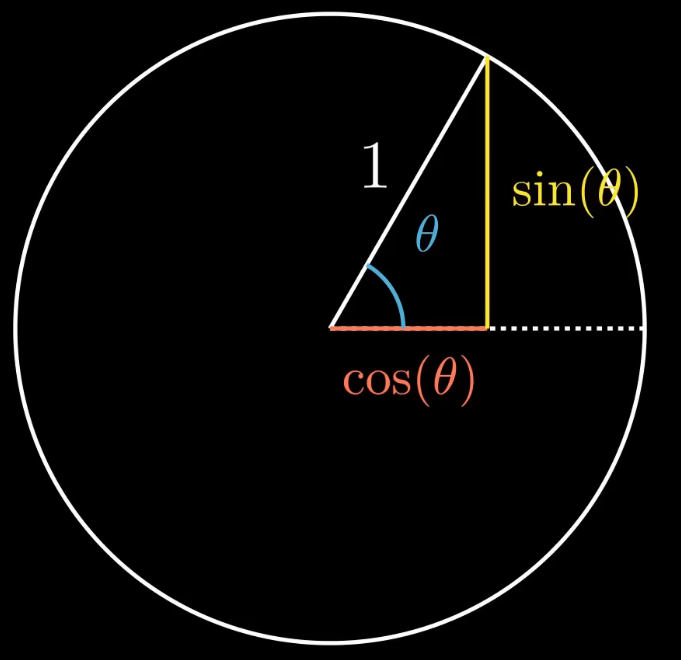
\includegraphics[scale=0.3]{./images/theta}
\par
}

Pues se dice que el {\large $\sin$} es la longitud del lado amarillo,
mientras que la del lado rojo es el {\large $\cos$}. Si variamos el
valor de {\large $\theta$} las longitudes de estos segmentos cambian, se hacen mas grandes y mas pequeños. Es decir, esto depende del ángulo
{\large $\theta$} y por lo tanto, podemos dibujar cuanto valen el
	{\large $\sin$} y el {\large $\cos$} en función.\\
\par

{
	\centering
	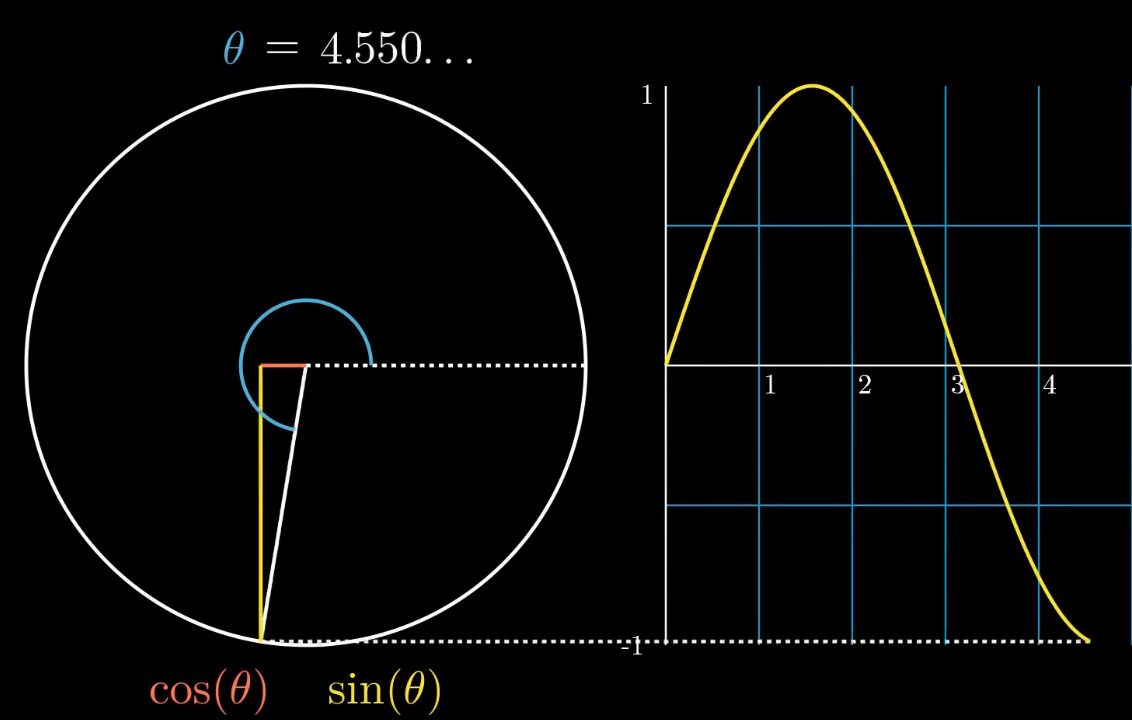
\includegraphics[scale=0.3]{./images/function}
	\par
}

Todo esto esta correcto, pero ahora
\textbf{¿Qué que pasa si quiero calcular el seno de algo
	con muchos decimales?} Como $2.4521352121....$\\

La respuesta lógica es que podríamos aumentar la precisión de las
medidas y obtendríamos el resultado ¿No? Pues no es tan simple, ya
que no tenemos algo como "precisión suficiente" ya que son muchos
decimales. Pero las calculadoras lo hacen ¿Verdad?\\
\par

\textbf{¿Como lo hacen las calculadoras?}\\
Ya que es imposible de almacenar en la memoria de las calculadoras todos
los valores del seno para todos los valores que se introduzca, suelen
calcularlo de dos formas diferentes. La primera, un algoritmo muy famoso
llamado \textbf{Cordic} y por las segunda, las \textbf{Series de Taylor}.
\\
\\

\subsection{¿Que son las series de Taylor?}

Las series de Taylor son representaciones de funciones mediante una suma infinita de términos calculados a partir de las derivadas de la función en un único punto. Permiten aproximar funciones complicadas con polinomiosmás manejables.\\

{\large\textbf{Definición Formal}}\\
Sea $f(x)$ una función infinitamente derivable en un punto $a$. La serie de Taylor de $f(x)$ centrada en $a$ es:

\begingroup
\Large
\begin{equation*}
	f(x) = \sum_{n=0}^\infty \frac{f^n(a)}{n!}(x-a)^n
\end{equation*}
\endgroup

Donde:
\begin{itemize}
	\item $f^n(a)$: es la derivada n-ésima de $f$ evaluada en $a$.
	\item $n!$: es el factorial de $n$.
	\item $(x-a)^n$: es la potencia n-ésima del desplazamiento respecto a $a$
\end{itemize}

\subsection{¿Para que sirven?}
Las series de Taylor se utilizan para:
\begin{itemize}
	\item Aproximar funciones difíciles de calcular(como $e^x$, $sin(x)$, $ln(x)$, etc).
	\item Resolver ecuaciones diferenciales.
	\item Realizar cálculos numéricos en ingeniería y física.
	\item Analizar el comportamiento local de funciones.
\end{itemize}

\subsection{¿Cómo se calcula una Serie de Taylor?}
Pasos:
\begin{enumerate}
	\item Elige el punto de desarrollo $a$
	\item Calcula las derivadas sucesivas de $f(x)$
	\item Evalúa esas derivadas en $a$
	\item Sustituye en la fórmula:
\end{enumerate}
\begingroup
\Large
\begin{align*}
	f(x) & \approx f(a) + f^\prime(a)(x-a) + \frac{f^{\prime\prime}(a)}{2!}(x-a)^2            \\
	     & + \frac{f^{\prime\prime\prime}(a)}{3!}(x-a)^3 + \frac{f^{(4)}(a)}{4!}(x-a)^4 + ... \\
\end{align*}
\endgroup

\subsection{Ejemplo}
a) Calcula la Serie de Taylor de $f(x)=x^4-3x^2+1$, alrededor de $x_0$ = 1
\begin{itemize}
	\item Calcular las derivadas sucesivas de $f(x)$
	      \begingroup
	      \Large
	      \begin{align*}
		      f(x)       & = x^4 - 3x^2 + 1 \\
		      f'(x)      & = 4x^3-6x        \\
		      f''(x)     & = 12x^2-6        \\
		      f'''(x)    & = 24x            \\
		      f^{(4)}(x) & = 24             \\
		      f^{(5)}(x) & = 0
	      \end{align*}
	      \endgroup

	\item Evaluar las derivadas en $a$
	      \begingroup
	      \Large
	      \begin{align*}
		      f(1)       & = -1 \\
		      f'(1)      & = -2 \\
		      f''(1)     & = 6  \\
		      f'''(1)    & = 24 \\
		      f^{(4)}(1) & = 24 \\
		      f^{(5)}(1) & = 0  \\
	      \end{align*}
	      \endgroup

	\item Sustituir en la fórmula
	      \begingroup
	      \Large
	      \begin{equation*}
		      f(x) \approx f(a) + f^\prime(a)(x-a) + \frac{f^{\prime\prime}(a)}{2!}(x-a)^2 + ...
	      \end{equation*}\\
	      \large
	      \begin{align*}
		      f(x) & = -1-2(x-1) + \frac{6}{2!}(x-1)^2 +\frac{24}{3!}(x-1)^3+
		      \frac{24}{4!}(x-1)^4                                                             \\
		      f(x) & = -1-2(x-1)+\frac{6}{2}(x-1)^2 +\frac{24}{6}(x-1)^3+ \frac{24}{24}(x-1)^4 \\
		      f(x) & = -1-2(x-1)+3(x-1)^2+4(x-1)^3+(x-1)^4
	      \end{align*}
	      \endgroup

	\item Entonces la serie de Taylor es:
	      \begingroup
	      \Large
	      \begin{equation*}
		      f(x) = -1-2(x-1)+3(x-1)^2+4(x-1)^3+(x-1)^4
	      \end{equation*}
	      \endgroup
\end{itemize}

\newpage
\begin{center}
	\section{Representación de Funciones Mediante Series de Taylor}
\end{center}
\subsection{Introducción}
La representación de funciones mediante series de Taylor es una de las herramientas más importantes del análisis matemático. Esta técnica permite aproximar funciones complejas utilizando polinomios infinitos, lo que resulta de gran utilidad en diversos campos como la física, la ingeniería, la economía y la informática. \\

En matemáticas, una serie de Taylor de una función $f(x)$ infinitamente derivable (real o compleja) definida en un intervalo abierto $(a-r, a+r)$ \\

Si esta serie converge para todo $x$ perteneciente al intervalo $(a-r, a+r)$ y la suma es igual a $f(x)$, entonces la función $f(x)$ se llama analítica. Para comprobar si la serie converge $a f(x)$, se suele utilizar una estimación del resto del teorema de Taylor. Una función es analítica si y solo si se puede representar con una serie de potencias; los coeficientes de esa serie son necesariamente los determinados en la fórmula de la serie de Taylor. \\

Si $a = 0$, a la serie se le llama serie de Maclaurin. \\

Esta representación tiene tres ventajas importantes:\\
La derivación e integración de una de estas series se puede realizar término a término, que resultan operaciones triviales.
Se puede utilizar para calcular valores aproximados de la función.
Es posible demostrar que, si es viable la transformación de una función a una serie de Taylor, es la óptima aproximación posible.

\subsection{Condiciones de Validez Para Series de Taylor}
No todas las funciones se pueden representar por su serie de Taylor en todo su dominio. Para que una función $f(x)$ sea representada por su serie de Taylor en un intervalo alrededor de $a$, se deben cumplir ciertos requisitos:
\begin{itemize}
	\item $f(x)$ debe ser infinitamente derivable en ese intervalo
	\item La serie debe converger
	\item El valor al que converge la serie debe ser igual al valor real de la función (convergencia uniforme o convergencia absoluta en algunos casos).
\end{itemize}
\end{document}
